\documentclass[dvisvgm]{standalone}
\usepackage{tikz}
\usepackage{amsmath}
\usepackage{amsfonts}

\begin{document}
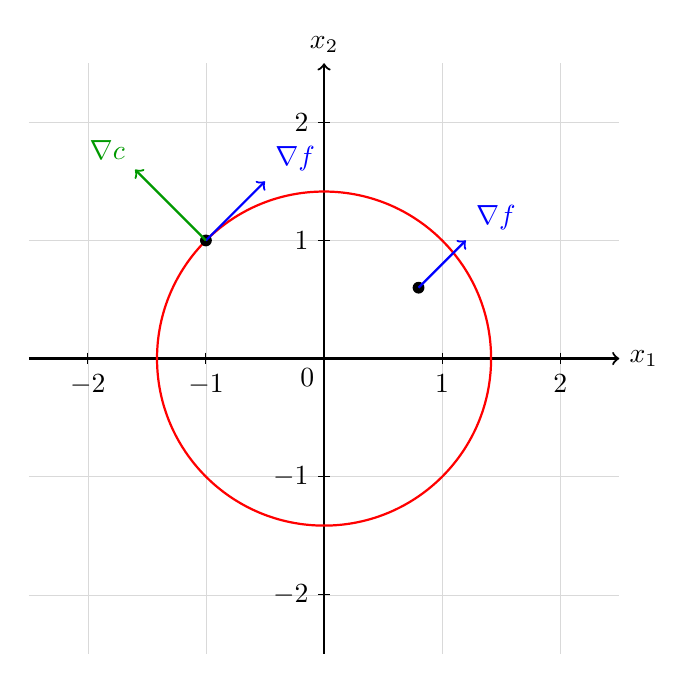
\begin{tikzpicture}[scale=1.5]
    % Grid
    \draw[help lines, gray!30] (-2.5,-2.5) grid (2.5,2.5);
    
    % Axes
    \draw[thick,->] (-2.5,0) -- (2.5,0) node[right] {$x_1$};
    \draw[thick,->] (0,-2.5) -- (0,2.5) node[above] {$x_2$};
    
    % Origin
    \node[below left] at (0,0) {$0$};
    
    % Tick marks
    \foreach \x in {-2,-1,1,2} {
        \draw (\x,0.05) -- (\x,-0.05) node[below] {$\x$};
        \draw (0.05,\x) -- (-0.05,\x) node[left] {$\x$};
    }
    
    % Constraint circle: x1^2 + x2^2 = 2
    \draw[thick, red] (0,0) circle ({sqrt(2)});
    

    
    % Point on the circle
    \fill[black] ({sqrt(2)*cos(135)},{sqrt(2)*sin(135)}) circle (0.05);
    \coordinate (P1) at ({sqrt(2)*cos(135)},{sqrt(2)*sin(135)});
    
    % Point inside the circle
    \fill[black] (0.8,0.6) circle (0.05);
    \coordinate (P2) at (0.8,0.6);
    
    % Gradient of objective function f at point on circle
    \draw[->, thick, blue] (P1) -- ++(0.5,0.5) node[above right] {$\nabla f$};
    
    % Gradient of objective function f at point inside circle
    \draw[->, thick, blue] (P2) -- ++(0.4,0.4) node[above right] {$\nabla f$};
    
    % Gradient of constraint c at point on circle
    \draw[->, thick, green!60!black] (P1) -- ++({2*sqrt(2)*cos(135)*0.3},{2*sqrt(2)*sin(135)*0.3}) node[above left] {$\nabla c$};
    

    
\end{tikzpicture}
\end{document}
